\chapter{Metoder}
Dette kapitel indeholder beskrivelser af hvordan projektet er udført, og hvilke metoder, der er brugt. Yderligere indeholder kapitlet projektstyring, samt hvilke modeller, der er fulgt igennem projektforløbet. 

\section{Samarbejdsaftale}
For at sikre gruppens enighed i udførelse af projektet, om blandt andet arbejdsindsats samt timer der skulle bruges på projektet blev der udarbejdet en samarbejdsaftale. Samarbejdsaftalen bevirker derfor som en forventningsafstemning. Se samarbejdsaftalen i bilag \ref{bilag:samarbejdsaftale}

\section{Samarbejdspartnere}
Gruppens kunde er Søren Gregersen, overlæge på Medicinsk Endokrinologisk Afdeling, Aarhus Universitetshospital. Det er i samarbejde med Søren, at projektet er blevet specificeret, samt hvilke krav der er til den endelige prototype.
Samuel Alberg Thrysøe er gruppens projektvejleder. Der er afholdt ugentlige vejledermøder, hvor gruppen har givet status på projektet og hvor der er diskuteret forskellige problemstillinger. Til hvert vejledermøde har der været dagsorden med punkter, som formål og begrundelse for punkterne på dagsorden. Dagsordenerne er sendt til vejleder senest en dag før vejledermødet. Dette er gjort for at give vejleder en chance for at forberede sig på den givne dagsorden. Til hvert vejledermøde er der udført et referat som kan ses i bilag \ref{modevejleder}.
Simon Vammen Grønbæk og Karl-Johan Schmidt har fungeret som projektets reviewgruppe. Der er holdt møde hver tredje uge omhandlende aftalt dagsorden. Formålet med review gruppen er at få konstruktiv feedback på evt. rettelser, opbygning af rapport og generel forståelse. Reviewgruppen har været gode til at sparre med omkring diskussioner, samt andre spørgsmål i gruppen. Dette har det været med til at drive projektet igennem de forskellige udviklingsfaser, da reviewgruppen også har været afhængige af datoen.

Reviewsmøderne har forgået ved, at grupperne har udvekslet dokumenterne, der skulle reviews. Grupperne har skrevet kommentar til dokumentet, hvorefter kommentarene og rettelserne er diskuteret på møderne. 

\newpage
\section{Udviklingsværktøjer}
Dette afsnit består af en kort beskrivelse omkring udviklingsværktøjer brugt i projektet.

\textbf{MATLAB:} Softwaren til systemet er udviklet i MATLAB. Versionen, der er anvendt, er R2015b. Tilføjelsespakker brugt i projektet er følgende:
\begin{itemize}
\item Arduino Support Package (14.2.2)
\item Webcam Support Package (15.2)
\end{itemize}
Disse pakker anvendes til at interagere med Arduinoen og USB mikroskopet. 

\textbf{Fritzing:} Fritzing er brugt til at illustrere kredsløbsdiagrammer(schematics), samt enhedstest af hardwaren ved illustrationer af \textit{fumlebræt}. Dette har bidraget til dokumentationen af  enhedstestene. Derudover har det givet mulighed for at opstillingerne brugt på \textit{fumlebræt}, let kunne genskabes.

\textbf{Eagle:} Eagle er et program til udarbejdelse af print layouts. \textit{Eagle} er brugt til at lave et samlet PCB layout for hardwareelementerne. I \textit{Eagle} er der generet Gerber-filer, som er sendt til PCB fabrikanten.

\textbf{SolidWorks:} SolidWorks er et program til at illustrere mekaniske 3D modeller med.  \textit{SolidWorks} er brugt til at lave kamerahuset med for senere at få det 3D printet.

\textbf{Arduino IDE:} Programmet som er udbudt af \textit{Arduino} bruges til at programmere \textit{Arduino} udviklingskortet. \textit{Arduino IDE} er i projektet brugt til enhedstest for at teste hardware opstillingerne. 

\textbf{Microsoft Visio:} Microsoft Visio er et tegne program, som bruges til at illustrere forskellige modeller. Programmet er valgt til at lave udviklingsdiagrammer, samt illustrationer med. 

\textbf{Texmaker:} Dette program er brugt til at skrive alt dokumentationen i projektet. \textit{Texmaker} gør det muligt at arbejde på samme dokument samtidigt, hvilket har været en stor hjælp.

\textbf{PivotalTracker:} PivotalTracker er et scrumbaseret projektstyringsværktøj, der hjælper med at styre arbejdsressourcerne i projektet. Der er i afsnittet \ref{subsec:agil} uddybet hvordan \textit{PivotalTracker} er brugt i projektet.

\textbf{GitHub:} Er et versionsstyringsprogram, som i projektet er brugt til versionsstyring af dokumenter og \textit{Matlab} koden til projektet. Se afsnit \ref{subsec:github} for uddybende dokumentation omkring hvordan \textit{Github} er brugt.

\textbf{Dropbox:} Det cloudbaserede delingsværktøj \textit{Dropbox} er i projektet brugt til at gemme og dele artikler, diagrammer, billeder og generelle noter.

\textbf{Microsoft Onenote:} Onenote er et program til at lave noter i. I projektet er programmet brugt til at have fælles noter og huskelister.


\newpage
\section{Versionsstyring}
I projektet er der gjort brug af versionsstyringssoftwaren \textit{GitHub}. Til store ændringer har dokumenterne fået et nyt versionsnummer og versionshistorikstabellen er opdateret i hvert dokument, se tabellen nedenfor. 

\begin{center}
		\begin{longtable}{ | m{1.5cm} | m{2cm}| m{7cm}| m{2cm}| } 
			\hline
			\textbf{Version}  & \textbf{Dato} & \textbf{Beskrivelse} & \textbf{Initialer}  \\ 
			\hline
			0.1  &  19/09 2015  & Dokument sendt til review & AE og AT \\
			\hline
		1.0  &  19/09 2015  & Rettelser fra reviewmøde og Latex layout & AE og AT \\
		\hline
		1.1  &  20/10 2015  & Kamerakrav tilføjet & AE og AT \\
		\hline
		2.0  &  6/11 2015  & Definitioner og layout ændringer & AE og AT \\
			\hline
		\end{longtable}
		
	\end{center}


\subsection{Github}
\label{subsec:github}
Til versionsstyring af projektdokumentationen og source kode anvendes GitHub, som bygger på open source versionsstyringssystemet Git. Her opdateres der løbende ændringer, så det nyeste dokumentation og source kode altid er tilgængeligt. 
Som user interface til GitHub anvendes GitHub Desktop (figur: \ref{fig:git}). I GitHub Desktop vises en tidslinje, for hvornår, der er lavet ændringer. Under de enkelte filer kan det observeres, hvad der er ændret i for den gældende version. Programmet giver yderligere indblik, i hvilke filer, der lokalt er lavet ændringer i, som ikke er tilføjet repositoriet endnu.
\begin{figure}[H]
	\centering
	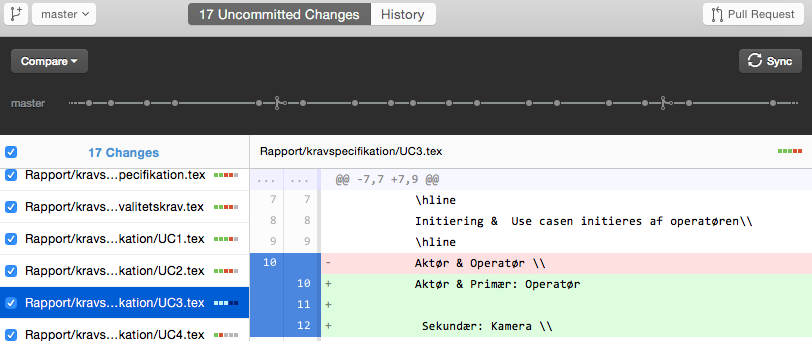
\includegraphics[width=1\textwidth]{billeder/github.png}
	\caption{GitHub Desktop}
	\label{fig:git}
\end{figure}
\newpage

\section{Projektstyring} 
Til projektstyring er der brugt en stage gate model. En stage gate model(figur \ref{fig:stage-gate}) er bestående af nogle udviklingsfaser(stages), hvor der er en deadline for de konkrete faser. For at komme til næste fase/stage, skal der være opfyldt nogle kriterier. Kriterierne opstilles i en tjekliste(se figur \ref{fig:stage-gate-tjekliste}), hvor de kan krydses af. Alle punkter skal være opfyldt for at komme igennem gaten. En stage gate model er god til at få et produkt på markedet, men det har sine svagheder ved en agil udviklingsprocess. Derfor er der i projektet arbejdet med åbne gates, hvilket gør det muligt at gå tilbage for at justere på dokumenter. I projektet er stage gate modellen brugt som tidsplan og en metode, der har været med til at sikre, at fasen var færdig inden næste fase igangsættes. 

%\begin{landscape}
\begin{figure}[H]
	\centering
	\includegraphics[width=0.65\textwidth]{billeder/Hovedrapport/Stage-gatel.PDF}
	\caption{Stage gate model}
	\label{fig:stage-gate}
\end{figure}
%\end{landscape}

\begin{figure}[H]
	\centering
	\includegraphics[width=0.7\textwidth]{billeder/Hovedrapport/Stagegatetjekliste.PDF}
	\caption{Stage gate tjekliste}
	\label{fig:stage-gate-tjekliste}
\end{figure}

%\begin{sidewaysfigure}
%\begin{figure}[H]
%	\centering
%	\includegraphics[width=0.6\textwidth]{billeder/Hovedrapport/Stage-gateP.PDF}
%	\caption{Stage gate model}
%	\label{fig:moscow}
%\end{figure}
%\end{sidewaysfigure}



%\begin{figure}
%  \begin{sideways}
%    \begin{minipage}{27.5cm}
%      \includegraphics[width=0.6\textwidth]{billeder/Hovedrapport/Stage-gateP.PDF}
%    \end{minipage}
%  \end{sideways}
%  \centering
%  \caption[Caption]{Caption.}
%  \label{pic:picture}
%\end{figure}

\subsection{Agil udviklingsproces}
\label{subsec:agil}
I projektet er der brugt en agil arbejdsproces hvor der konstant er fokus på at målrette og prioritere arbejdet, der giver mest værdi for projektet og kunden. Derfor er der løbende prioriteret mellem opgaverne, hvorefter delopgaverne er blevet revurderet og planlagt. Dette gør at produktet og resultater evalueres og testes løbende, hvilket danner grundlag for prioriteringen af opgaverne til næste periode(sprint). Til at sikre arbejdsressourcerne tilrådighed for projektet er brugt på den mest effektive måde, er der valgt at bruge elementer fra SCRUM. SCRUM er en iterativ arbejdsmetode, hvor  der er iterationer(sprints), som i dette projekt har haft en periode på en uge. SCRUM er implementeret i projektet vha. \textit{Pivotaltracker}. 

I Pivotaltracker defineres projektets arbejdsopgaver, hvorefter de tildeles point alt efter hvor stor arbejdsbyrden er. De enkelte opgaver prioriteres herefter i projektets backlog, hvor Pivotaltracker automatisk tilføjer opgaver til den igangværende sprint udfra den nuværende “velocity”. Et nyt sprint påbegyndes automatisk når en ny uge starter.

Det betyder, at der er fuldstændig styr på om projektet går for langsomt, eller om udviklingen af projektet er godt med. Dette kan holdes op imod den tidligere nævnte stage gate model.

Herudover giver Pivotaltracker mulighed for en komplet log over projektets udførte opgaver og afsluttede sprints. Her kan man se hvilke opgaver, der er udført i hvilken uge. I projektet anvendes dette som logbog for udførte arbejdsopgaver. Se logbøgerne fra \textit{Pivotaltracker} i bilag \ref{bilag:Logboger}.

En opgave kan have forskellige states, som definerer dens status. Når en opgave er afsluttet kan den afleveres til review, hvor den herefter enten kan godkendes eller afvises. Dette er særligt anvendeligt i projektets udviklingsfase, hvor en feature kan testes og godkendes af et andet projektmedlem. Figur \ref{fig:pt_sprints}  viser et overblik over tidligere sprints, hvor figur \ref{fig:pt_currentsprint} viser en igangværende sprint med godkendte, afsluttet og endnu ikke færdiggjorte opgaver.

\begin{figure}[htbp] \centering
\begin{minipage}[b]{0.48\textwidth} \centering
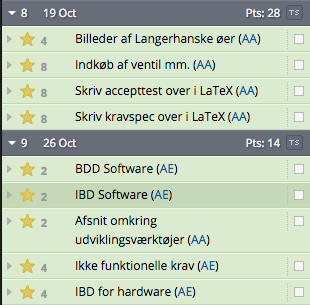
\includegraphics[width=1.00\textwidth]{billeder/pt_previous_sprints} % Left picture
\end{minipage} \hfill
\begin{minipage}[b]{0.48\textwidth} \centering
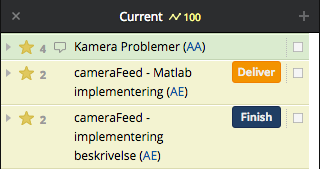
\includegraphics[width=1.00\textwidth]{billeder/pt_current_sprint} % Right picture
\end{minipage} \\ % Captions og labels
\begin{minipage}[t]{0.48\textwidth}
\caption{To færdiggjorte sprints} % Left caption and label
\label{fig:pt_sprints}
\end{minipage} \hfill
\begin{minipage}[t]{0.48\textwidth}
\caption{Igangværende sprint} % Right caption and label
\label{fig:pt_currentsprint}
\end{minipage}
\end{figure}

\section{Udviklingsfaserne}
Under udviklingen af projektet er der gennemgået fire faser. Den første fase i projektet har været konceptanalyse. Konceptanalysen bestod bl.a. af litteratursøgning omkring langerhanske øer, dette blev gjort for at opnå tilstrækkelig viden omkring størrelserne, deres egenskaber mm. Der blev også søgt efter allerede eksisterende sorteringsmetoder, som blev anvendt på det daværende tidspunkt. Dette var primært for at opnå erfaring inden for området på kort tid. Efter litteratursøgningen blev et overordnet koncept etableret i samarbejde med kunden(\textit{Søren Gregersen}). Ydermere er det i konceptanalysen, at der er identificeret problemstillinger og afgrænsninger af projektet. Samtidigt med konceptanalysen, blev der fokuseret på produktionen af produktet. Det er gjort for at undgå løsninger, som ikke kan produceres eller er besværlige at fremstille. Til sidst i konceptfasen er der udarbejdet en tidsplan for projektet.

Den anden fase består af kravspecifikationen, hvilket er udarbejdet i tæt samarbejde med kunden. En kravspecifikation har sikret at kunde og projektudviklere er enige om projektets udformning. I kravspecifikationen er der brugt usecasediagram, samt fully dressed beskrivelser af hver usecase. Der laves fully dressed, for at klaregøre normal forløbet for hver usecase, samt undtagelser og udvidelser til dem. Derudover er det også i kravspecifikationen. at der er specificeret ikke funktionelle krav og kvalitetskrav. Samtidigt med kravspecifikationen er der udarbejdet en accepttest. Denne test er med til at verificere at alle krav, der er bestemt i samarbejde med kunden, er opfyldte. I accepttesten er det beskrevet hvordan hver enkelt krav skal testes. Accepttesten udføres før produktet afleveres til kunden. Se afsnit \ref{subsec:krav} for eksempler.

Den tredje fase i projektet er designfasen, hvor der udfra kravspecifikationen er lavet overordnede diagrammer. Diagrammerne er brugt til at beskrive systemet, men også i mindre delsystemer. Det er diagrammerne, der er brugt til at videreudvikle systemet. Desuden er de enkelte komponenters specifikationer beskrevet i designdokumentet. Derfor er det i denne fase at komponenterne til projektet er bestilt. Se afsnit \ref{subsec:design} for eksempler. Efter denne fase var der dannet et overblik over hvilke opgaver der skulle implementeres. Derfor blev der udarbejdet en handlingsplan med en revurderet tidsplan for projektet, som kan ses i bilag \ref{bilag:Handlingsplan}. De primære dele af handlingsplanen består i at øge arbejdsressourcerne til 50 timer i ugen. hvilket også kan ses i \textit{PivotalTracker}, hvor målet for \textit{Velocity} har været 100 point. 

I den fjerde fase er der blevet produceret en prototype. Derfor er der i denne fase; kodet, monteret og testet. Denne fase er sket efter en iterativ proces, hvor der først kodes, monteres og derefter testes. Dette er gjort ved så små delelementer som muligt, for at sikre at hver delelement virker inden det sættes sammen. Se afsnit \ref{subsec:Implement} for eksempler af denne fase. 

De fire udviklingsfaser i projektet kan illustreres ligesom på figur \ref{fig:v-model}. Modellen har sine fordele og ulemper. Fordelene er, at der sikres dokumentation af projektet fra starten, samt at der hele tiden tænkes på slutresultatet og slutbrugeren. Ulemperne er, at der er meget dokumentation, der bliver ændret løbende. Dermed forekommer dette som spildtid, men det sikre samtidigt, at projektet bliver veldokumenteret og gennemtænkt fra starten.

\begin{figure}[H]
	\centering
	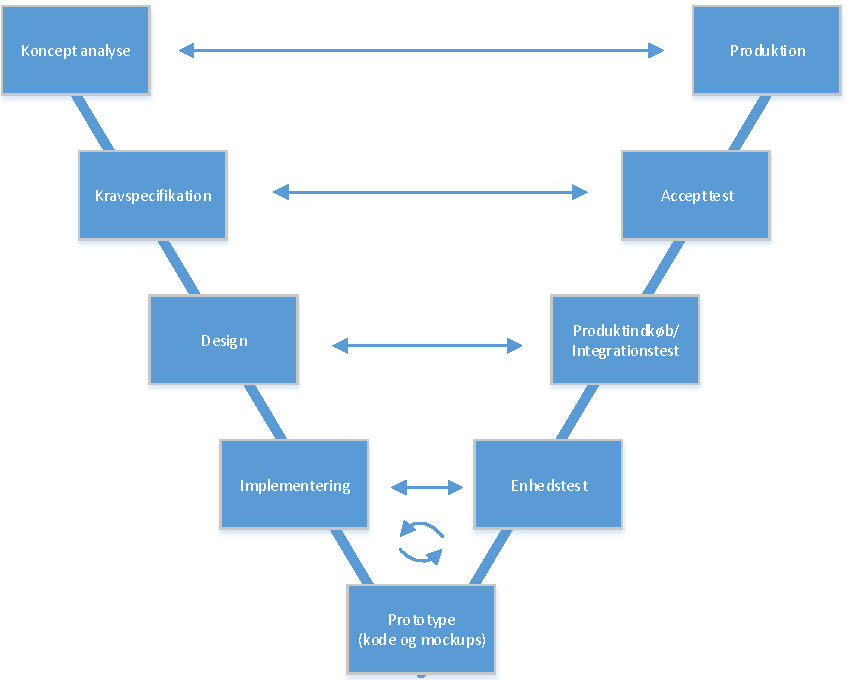
\includegraphics[width=0.7\textwidth]{billeder/Hovedrapport/V-model.PDF}
	\caption{V-model}
	\label{fig:v-model}
\end{figure}

I modsætning til v-modellen findes der også vandfaldsmodellen, hvor hver enkelt fase bliver lavet færdig før næste fase påbegyndes. Dette medfører ofte nedprioritering af test og andre sene deadlines i projektet, grundet at tidligere tidsplaner er overskredet. Det er derfor denne type model ikke er anvendt i projektet
\newpage

\section{Første udviklingsfase: Konceptanalyse}
For at eftervise at der er brugt de beskrevne metoder ovenfor, er der valgt at tage eksempler med i rapporten. I afsnittet er der eksempler fra hver af de fire udviklingsfaser. Den første fase er konceptanalysen, som primært har bestået af udarbejdning af forprojektet. I forprojektet er der kort defineret krav, bdd samt en projektplan for projektet. Projektplanen i koncept analysen kan ses på figur \ref{fig:forprojekt}

\begin{figure}[H]
	\centering
	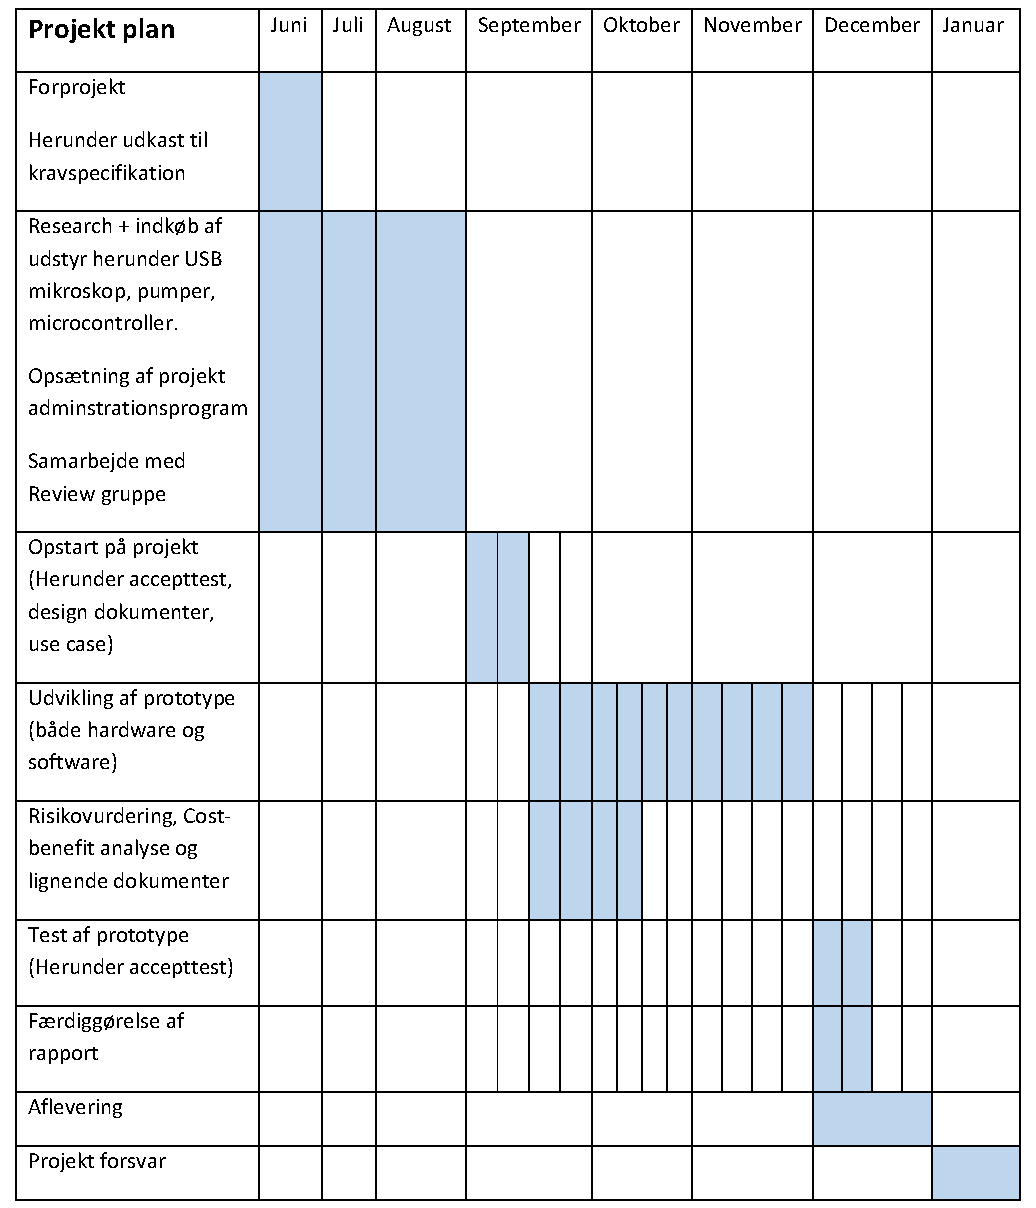
\includegraphics[width=0.9\textwidth]{billeder/Hovedrapport/forprojektplan.pdf}
	\caption{Projektplan i forprojektet}
	\label{fig:forprojekt}
\end{figure}
Det er blandt andet projektplanen på figur \ref{fig:forprojekt}, som har henledt til stage gate modellen. Til sidst har koncept analysen været med til at give et overblik over hvilke komponenter der kunne være anvendelige og burde undersøges til prototypen.
 
\section{Anden udviklingsfase: Kravspecifikation og accepttest}
\label{subsec:krav}
For at vise et eksempel for den anden udviklingsfase i projektet, er der valgt at tage \textit{Aktør beskrivelse}, \textit{use case diagram}, samt et \textit{fully dressed use case} og et udpluk fra accepttesten.


\subsection{Aktør beskrivelse}
Systemets primære aktør er operatøren, som står for påfyldning af celler, samt start og stop af sorteringsprocessen. Operatøren har mulighed for at interagere med systemet via en grafisk brugergrænseflade. Systemets sekundære aktør er kameraet og PC’ens filsystem. Kameraet er systemets interface til detektion af de Langerhanske øer. Filsystemet er hvor der løbende gemmes en log over sorteringsprocessen.
\newpage
\subsection{Use case Diagram}
I Use case diagrammet (figur: \ref{fig:usecase}) er der vist, hvilke use cases systemet \textit{The Cell Collector} består af. Yderligere er det vist, hvilke aktører der initierer de enkelte use cases. På venstre side er systemets primære aktør \textit{operatøren} vist, mens systemets sekundære aktører \textit{kamera} og \textit{database} er placeret i højre side. 

\begin{figure}[H]
	\centering
	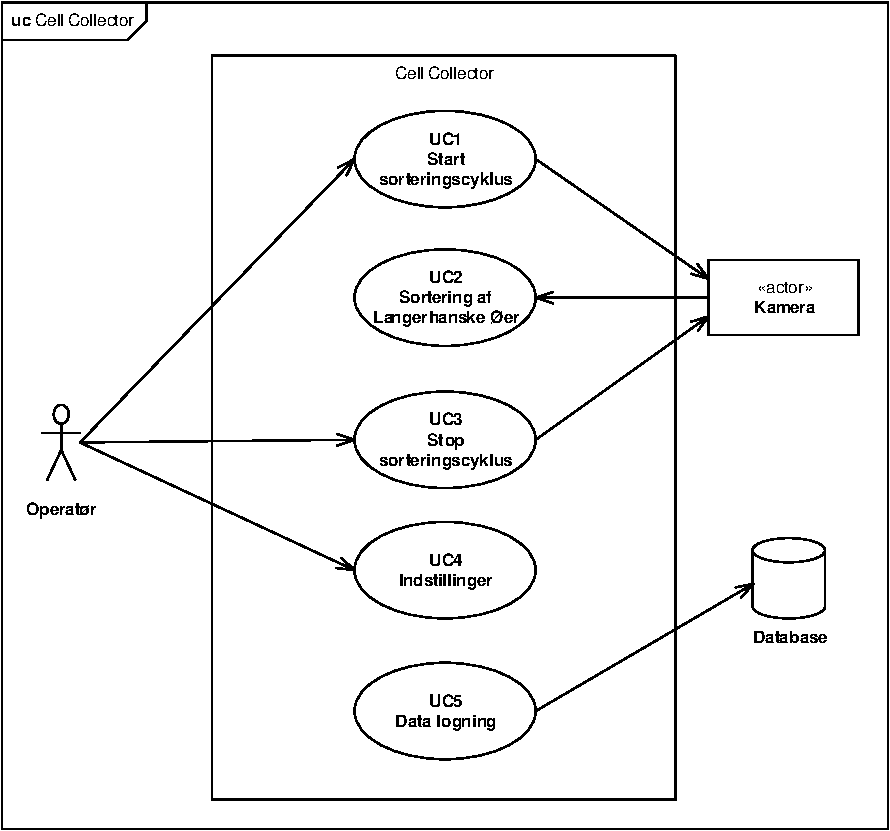
\includegraphics[width=1\textwidth]{billeder/UC_CellCollector.pdf}
	\caption{Use Case diagram for The Cell Collector}
	\label{fig:usecase}
\end{figure}

Efter use case diagrammet var færdigt, blev der udarbejdet fully dressed use cases, som kan ses på nedenstående tabel. Tabellen beskriver normalforløbet og undtagelser for \textit{Start af sorteringscyklus}. 

\newpage 
\subsection{Fully dressed use case for use case 1}
\begin{center}
		\begin{longtable}{ | m{4cm} | m{8cm}| } 
			\hline
			Mål & Start sorteringscyklus \\ 
			\hline
			Initiering &  Use casen initieres af operatøren\\
			\hline
			Aktør & 
			Primær: Operatør
			
			 Sekundær: Kamera			  \\ 
			\hline
			Startbetingelser & The Cell Collector programmet er startet på computeren \\ 
			\hline	
			Slutbetingelser ved succes & Systemet starter med sorteringen af Langerhanske øer \\
			\hline
			Slutbetingelser ved undtagelse & N/A \\
			\hline
			Normalforløb & \begin{enumerate}
				%\setlength\itemsep{0cm} % Decrease line distance
				\item Operatør fylder celleopløsningsbeholderen
				\item Celleopløsningsbeholderen er fyldt
				\item Operatør starter sorteringscyklus ved at klikke på [Start]
				\subitem [Undtagelse 1: Wastebeholder er fyldt] 
				\item Systemet initialiserer Arduinoen
				\subitem [Undtagelse 2: Ingen forbindelse til Arduino]
				\item Systemet kontrollerer celleopløsningsbeholderen ved at konvertere spændingen (\SI{}{\volt})  til \SI{}{\milli\litre}, og vise beholderens indhold (\SI{}{\milli\litre}) på GUI
				\item Systemet initialiserer kameraet
				\subitem [Undtagelse 3: Kameraet initialiserer ikke]
				\item Systemet tænder for kamera lyset
				\item Systemet tænder for pumpen
				
			\end{enumerate} \\ 
			\hline
			Undtagelser & [Undtagelse 1: Wastebeholder er fyldt] 
			
			\begin{enumerate}
			\item Systembesked: Tøm venligst Wastebeholder før start
			\item Operatøren trykker “OK”
			\item Systemet fortsætter opstartprocessen
			\end{enumerate} 
			
			[Undtagelse 2: Ingen forbindelse til Arduino]
			
			\begin{enumerate}
			\item 1.	Systembesked: Ingen forbindelse til Arduino, kontrollér forbindelser.
			\end{enumerate} 
	
			[Undtagelse 3: Kameraet initialiseres ikke]
			
			\begin{enumerate}
			\item System fejlmeddelse: Kameraet er ikke initialiseret:
			\item Genstart initialisering af Kameraet
			\end{enumerate} \\
			\hline
		\end{longtable}
		
	\end{center}

Efter at normalforløbet og undtagelserne er defineret, blev accepttesten lavet for den givne use case. Til hvert punkt i normalforløbet er der forberedt en test, som indeholder et \textit{krav nr}, \textit{handling} som beskriver hvad der skal gøres for at starte testen. Derudover er der \textit{forventet resultat}, som skal ske for at testen kan godkendes. \textit{Testmetode} beskriver hvordan testen skal udføres og hvordan den godkendes. Denne test er et udsnit af accepttesten, som er udarbejdet i samarbejde med kunden.

\subsection{Accepttest for krav 1.3}
	\begin{center}
		\begin{longtable}{ | m{4cm}| m{8.5cm}|} 
			\hline
			\textbf{Krav nr.} & 1.3    \\ 
			\hline
			\textbf{Handling} &  Operatør starter sorteringscyklus ved at klikke på [Start]  \\
			\hline
			\textbf{Forventet resultat} &  Opstartsprocessen igangsættes.  \\
			\hline
			\textbf{Testmetode}  & Knappen [Start] trykkes, observeres ved tekstboks på GUI, med teksten \textit{systemet starter op}.   \\
			\hline
			\textbf{Resultat}  &    \\
			\hline
			\textbf{Angiv godkendelse} &     \\
			\hline
			\textbf{Initialer} &     \\
			\hline
			\textbf{Dato} &    \\
			\hline
		\end{longtable}
	\end{center}
	
Resten af accepttesten for use casene kan ses i projektdokumentationen afsnit 2.2.

\section{Tredje udviklingsfase: Design}
\label{subsec:design}
I dette afsnit er der givet et eksempel på, hvordan projektet er gået fra krav til måder at løse projektet på. Der er blandt andet brugt BDD, IBD, flowchart samt sekvensdiagrammer til at beskrive funktioner og sammenhænge i projektet. 

\subsection{BDD og IBD for hardware}
Block definition diagram og interal block diagram over hardwaren er i projektet brugt til at sikre, hver hardware element kan kommunikere med hinanden. Yderligere er det med til at definere specifikationerne, for eksempelvis at indskærpe antallet af strømforsyninger.

Nedenstående BDD \ref{fig:bdd_Hardware} giver et overordnet overblik i, hvad \textit{The cell collector} indeholder af hardware elementer. Hierarkiet starter øverst med \textit{The cell collector}, som indeholder tre mindre hardware dele. Styreenheden, der er defineret som Arduino, indeholder bl.a. underelementet motordriver. Motordriveren indeholder yderligere tre dele,  det vil sige at pumpen, ventilen og kameralyset bliver styret her igennem. Udover styreenheden er der ikke elektriske dele, som beholdere og føringsveje til opløsningen med langerhanske øer. Den tredje underblok til \textit{The cell collector} er kameraet.

\begin{figure}[H]
	\centering
	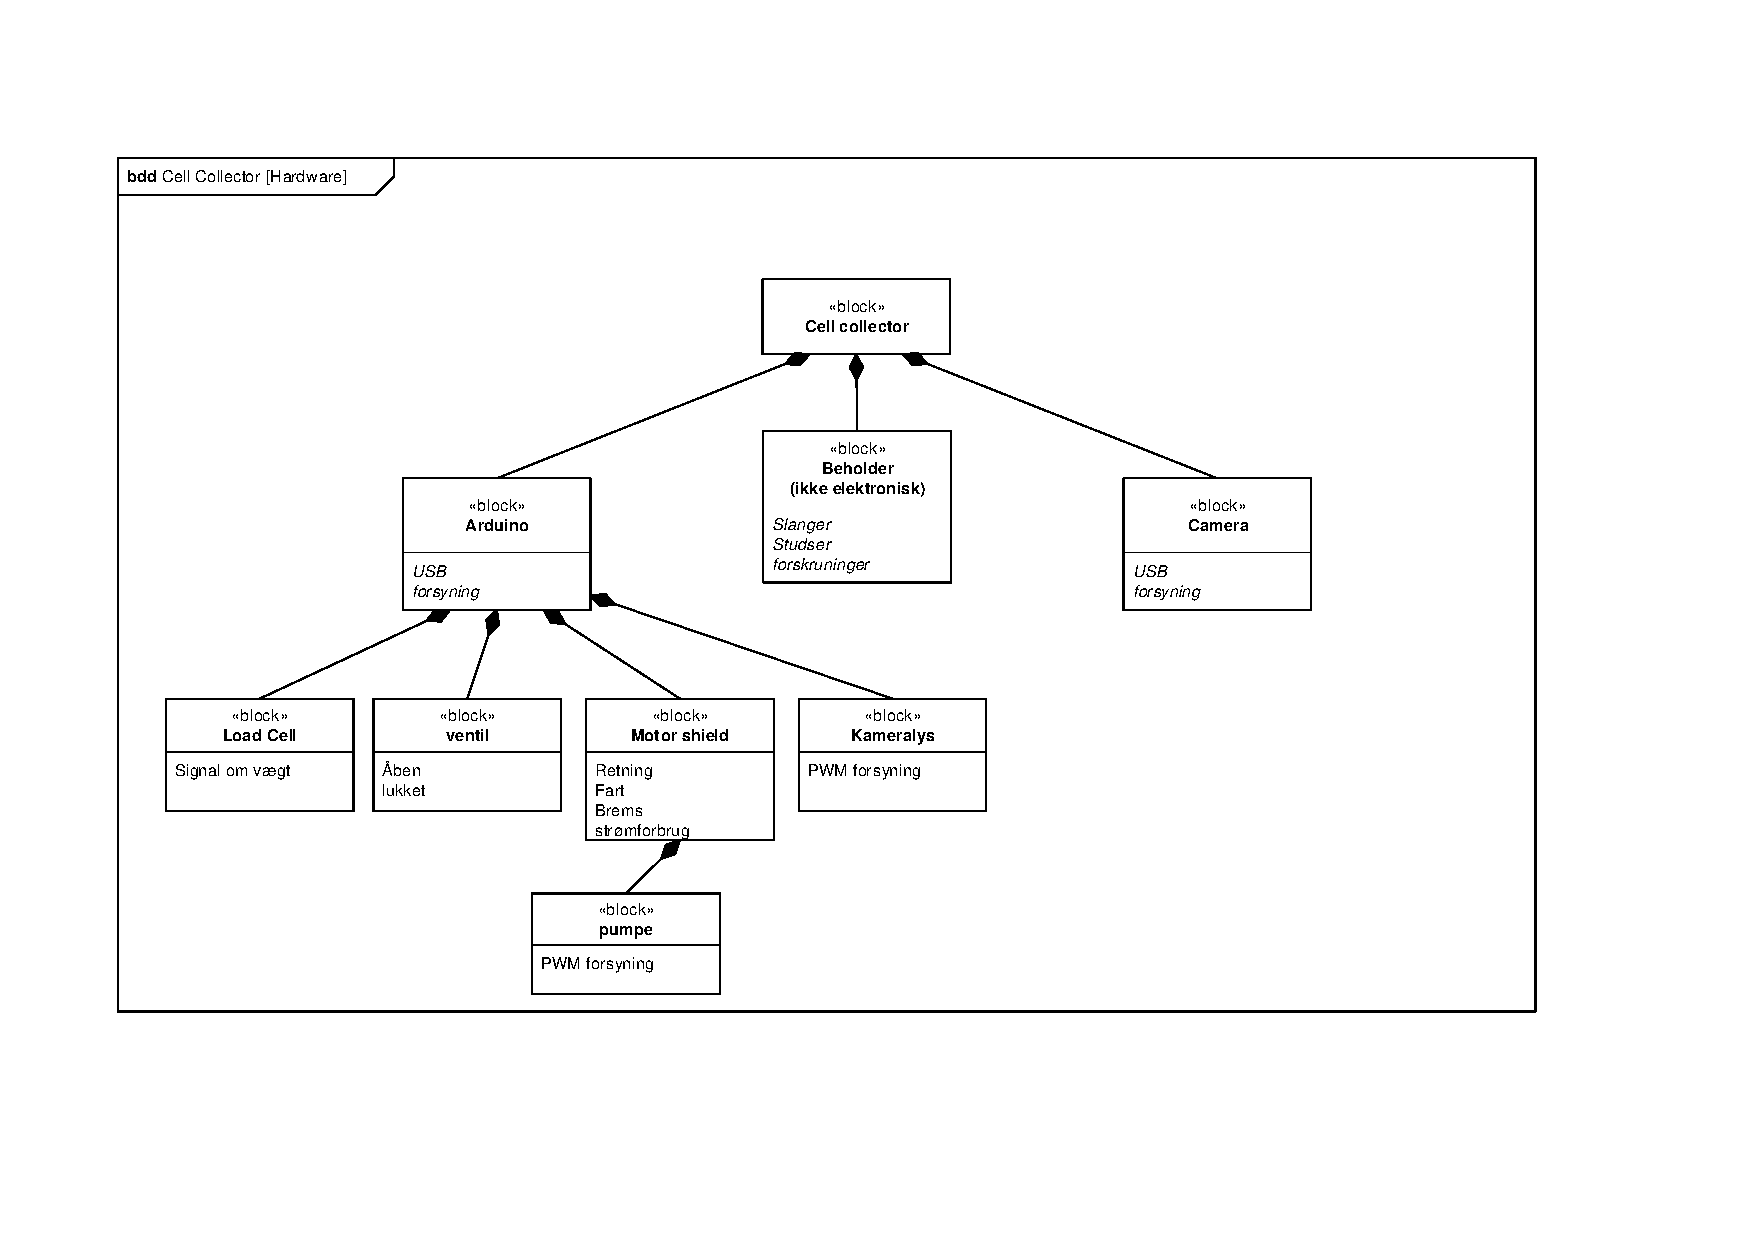
\includegraphics[width=1\textwidth]{pdf/BDD_Hardware.pdf}
	\caption{BDD - Cell Collector [Hardware]}
	\label{fig:bdd_Hardware}
\end{figure}

Nedenstående IBD figur \ref{fig:ibd_Hardware} beskriver mere præcist, hvordan de forskellige komponenter interagerer med hinanden. Diagrammet er brugt til, at der tidligt i udviklingsforløbet bliver defineret hvilke spændinger og signaltyper systemet skal indeholde. Systemet skal indeholde bestemte typer for, at kunne kommunikere med de interne dele.


\begin{figure}[H]
	\centering
	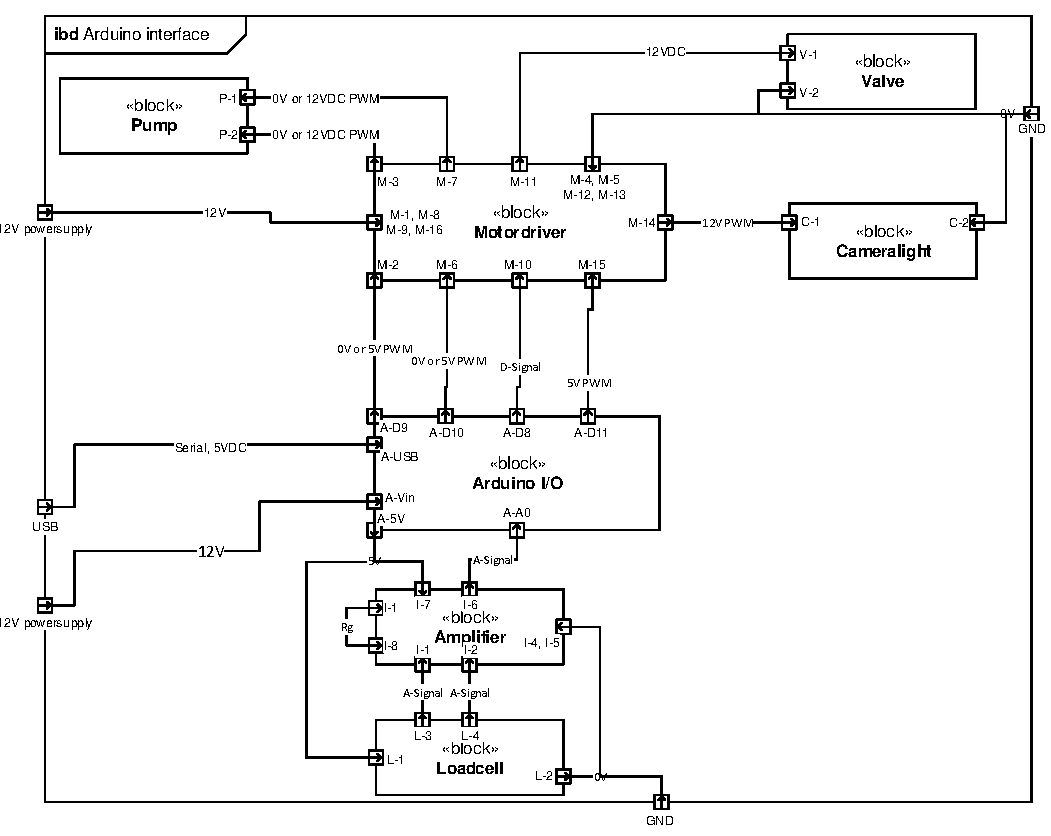
\includegraphics[width=1\textwidth]{pdf/IBD_Hardware(Arduino).pdf}
	\caption{IBD - Cell Collector [Hardware]}
	\label{fig:ibd_Hardware}
\end{figure}

Til ovenstående diagrammer er der udarbejdet tabeller som beskriver signalerne og de enkelte blokke (Se projektdokumentationen afsnit 3.3.4). fxnote{Tjek ref}

I designfasen er der udarbejdet specifikationer for de enkelte hardware dele, samt overvejelser omkring komponenten. 
\newpage
\subsection{Sekvensdiagrammer}
I designdokumentet er der yderligere lavet sekvensdiagrammer, hvilet giver overblik over de sekventielle dele af systemet til hver use case (se figur \ref{fig:sekvendisgr} for et eksempel). Sekvensdiagrammerne har været brugt til at klargøre, hvordan softwaren skal implementeres og i hvilken rækkefølge funktionerne skal eksekveres. Derudover har det været med til at danne et overblik over delene, der skal implementeres i projektet, samt dele arbejdsopgaverne op i mindre opgaver.
\begin{figure}[H]
	\centering
	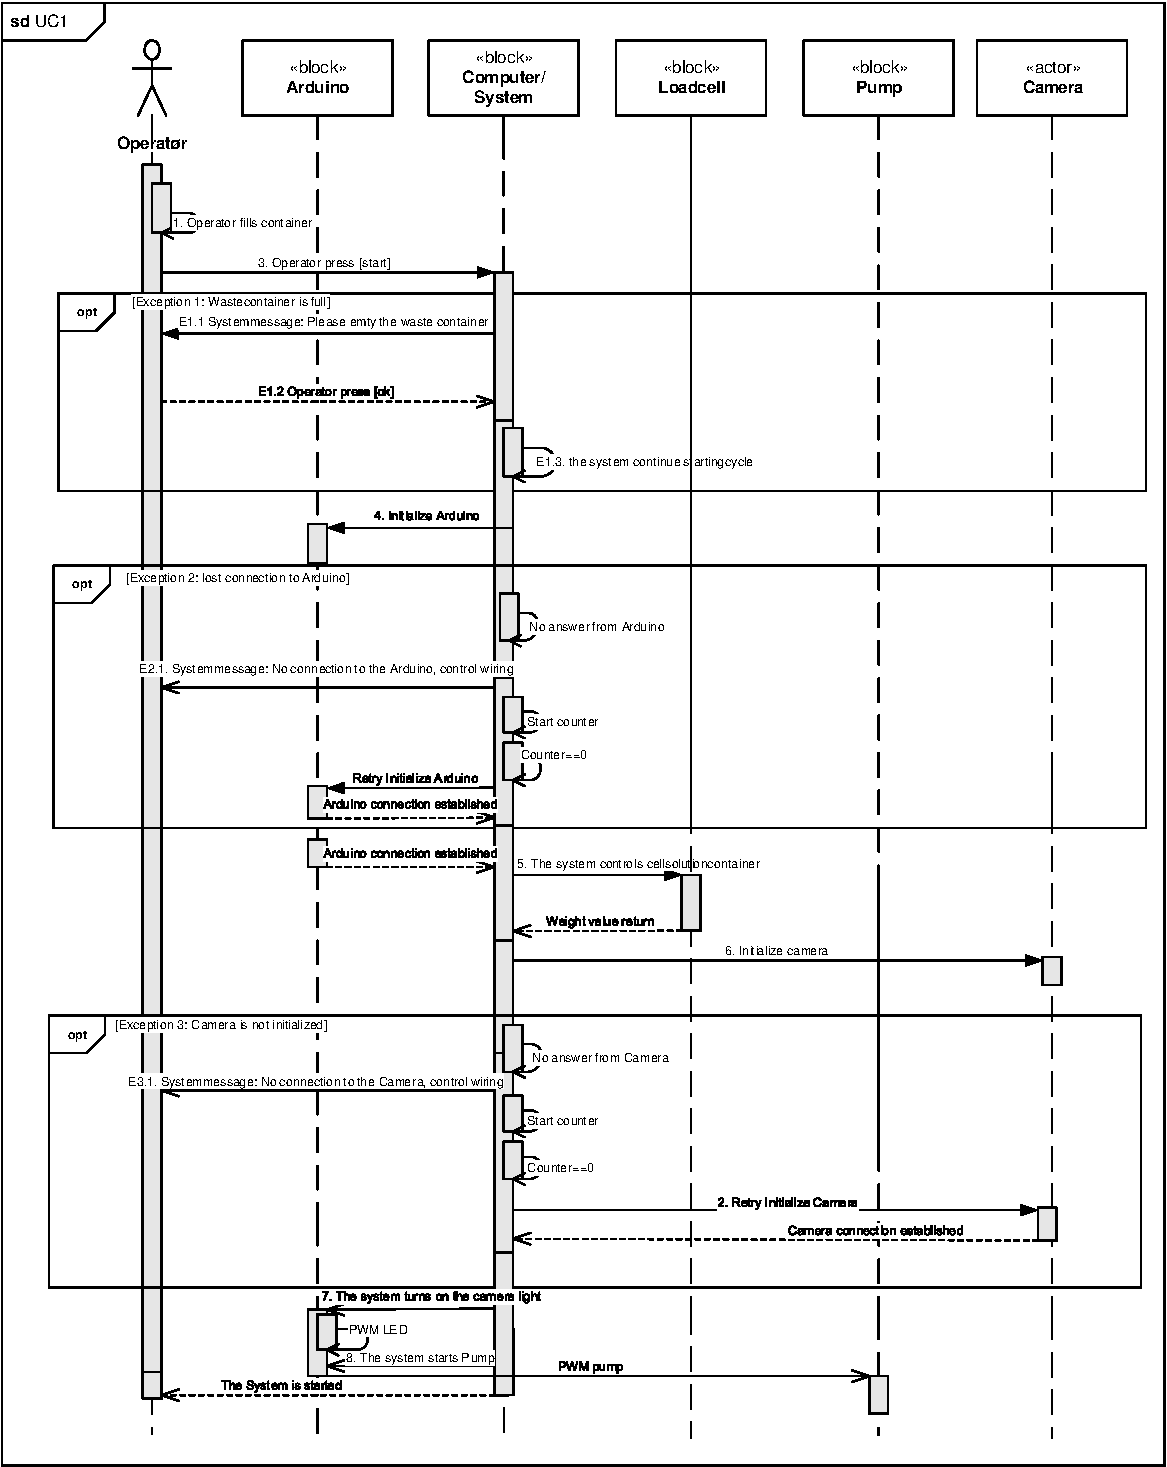
\includegraphics[width=1\textwidth]{pdf/UC1_cropped.pdf}
	\caption{Sekvensdiagram for usecase 1}
	\label{fig:sekvendisgr}
\end{figure}


\subsection{Vægtcelle}
Det følgende afsnit er et eksempel på, hvordan de enkelte hardware komponenter er blevet specificeret i designdokumentet, herunder de overvejelser, der er gjort. Afsnittet viser, hvordan vægtcellen er specificeret.

\label{subsec:loadcell}
Vægtcellen skal bruges til at kontrollere om, der er væske i celleopløsningsbeholderen. Systemet stopper sin sorteringscyklus, når der ikke længere er væske i celleopløsningsbeholderen.

\textbf{Specifikationer for Vægtcelle[\citet{DH7}]:} 
\begin{center}
		\begin{longtable}{ | m{6.5cm} | m{6.5cm}| } 
			\hline
			\textbf{Specifikation} &\textbf{Værdi} \\ 
			\hline
			\textbf{Max belastning:} & 1 kg \\ 
			\hline
			\textbf{Anbefalet arbejdsspænding} & 3-12V \\ 
			\hline
			\textbf{Output} & 1.0mV/V$\pm$0.15mV/V \\ 
			\hline
		\end{longtable}
\end{center}

Den indkøbte vægtcelle kan veje op til 1 kg, hvilket dækker vægten for celleopløsningsbeholderen på 250ml + beholderens vægt. I designfasen er der udarbejdet et teoriafsnit for at dokumentere den opnåede viden gruppen har fået. Designafsnittet indeholder desuden beregninger og kredsløbsdiagrammer. Det er illustreret i den overstående tabel, at vægtcellens output er i millivolt, hvilket har medført, at signalet skulle forstærkes. Dette er gjort vha. en operationsforstærker. For at vise et eksempel, er der trukket nedenstående afsnit ud fra designdokumentet (se projektdokumentation afsnit 4.2.1 \fxnote{Tjek ref} for hele afsnittet).

I databladet \ref{bilag:INA114} til INA114 vises det at den har en CMRR på 115dB, ved et gain på 1000 og en indgangsmodstand på 10G$\Omega$. Forstærkningen kan regnes ud fra formlen i databladet \ref{eq:gainina1}
\begin{align}
 G=(1+\frac{50K\Omega}{R_{G}})
 \label{eq:gainina1}
 \end{align} 
 I dette projekt skal der bruges et gain på $\frac{4,9V}{5mV}=980$, 4,9V for ikke at komme i mætning på arduinoens ADC og 5mV, da det er den maksimale spænding vægtcellen kan give, ved 5V forsyning.
 \begin{align}
 R_{G}=\frac{50k\Omega}{980-1}=51\Omega
 \label{eq:gainina2}
 \end{align}
Et gain på 980 giver en $NY_{Maksimalespænding}=980*5mV=4,9V \pm0,147V$, dvs at der nu er en opløsning på
\begin{align}
 \frac{1000g}{trin}=\frac{1000g}{1024}=0,977g/trin=>0,977*\frac{1024}{5V}=200g/V \pm30g
 \label{eq:gainina3}
 \end{align}
 
 Kredsløbet for INA114 og vægtcellen til arduinoen kan ses på figur \ref{fig:loadcelldiagram}.
 
  \begin{figure}[H]
	\centering
	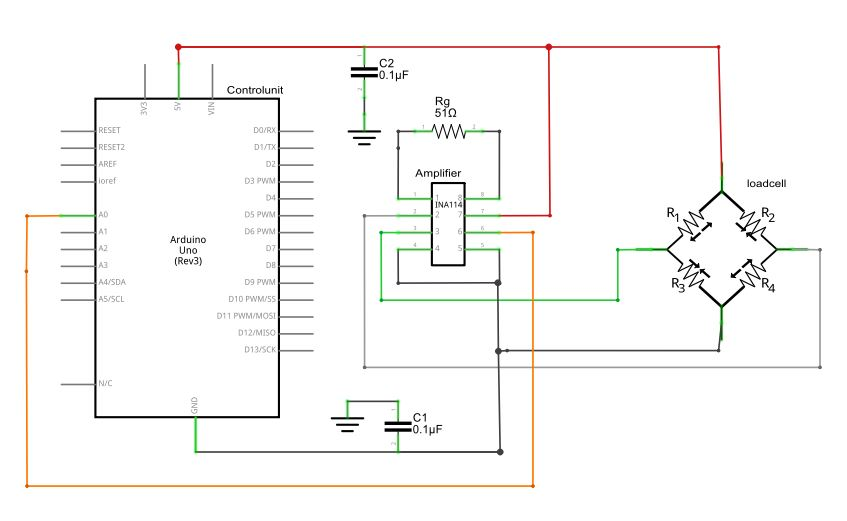
\includegraphics[width=0.9\textwidth]{billeder/Hardware/diagrammer/loadcelldiagram.JPG}
	\caption{Diagram for arduino, INA114 og vægtcelle}
	\label{fig:loadcelldiagram}
\end{figure}



\newpage
\section{Fjerde udviklingsfase: Implementering og enhedstest}
\label{subsec:Implement}
I dette afsnit er der vist et eksempel på hvordan vægtcellen er implementeret, både hardware-og softwaremæssigt. Til sidst i implementeringsfasen er der lavet en integrationstest. Integrationstesten for hardwaren er bestået af udarbejdelse i et shield til \textit{Arduinoen}. Da de enkelte faser er foregået ved en iterativ proces har det været mulighed at justere designdokumentet, hvis en komponent eller funktion blev implementeret anderledes end det var specificeret. På samme måde er designdokumentet ændret, hvis en enhedstest fejlede. Et eksempel på dette er kameraet, hvor det i enhedstesten viste sig at kvaliteten ikke var tilstrækkelig. Enhedstesten er vist i afsnit 4.3.1 i projektdokumentation.  \fxnote{tjek ref}

\subsection{Hardware}
Efter at diagrammet og kredsløbet er fastlagt i designdokumentet kunne vægtcellens kredsløb nu testes på et \textit{fumlebræt}. Se figur \ref{fig:loadcelltest} for testopstilling.

  \begin{figure}[H]
	\centering
	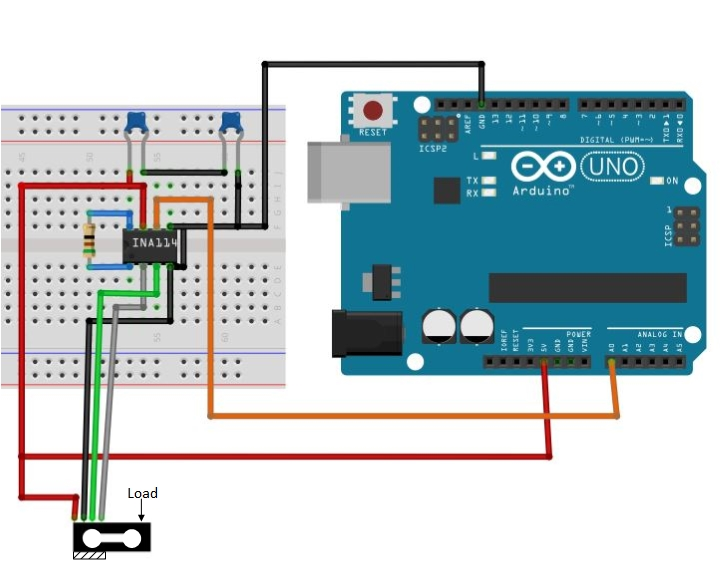
\includegraphics[width=0.9\textwidth]{billeder/Hardware/diagrammer/Drawing1.jpg}
	\caption{Test opstilling for vægtcelle}
	\label{fig:loadcelltest}
\end{figure}
De primære dele af test koden har været  \textit{sensorValue = analogRead(A0);} og \textit{Serial.println(sensorValue);}, hvor ved at inputtet på \textit{A0} er læst i \textit{serial monitor} som vist på figur \ref{fig:loadcell_test} ved langsom tømning af beholderen.

\begin{figure}[H]
	\centering
	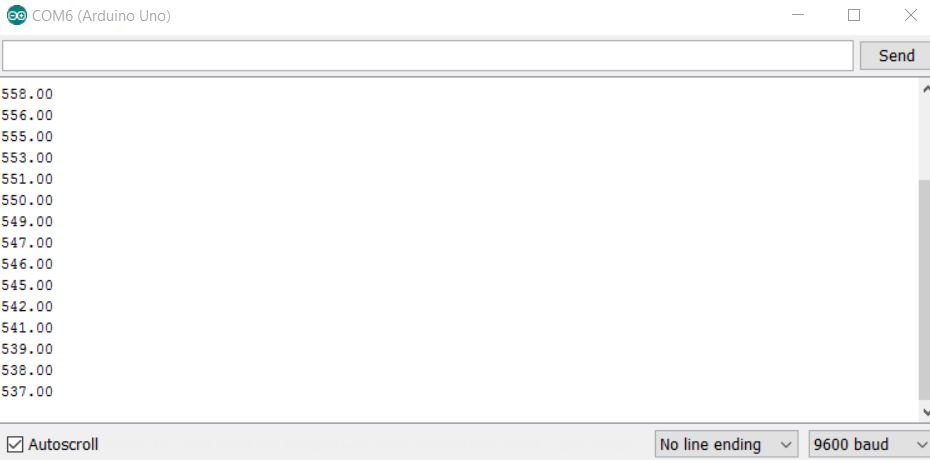
\includegraphics[width=0.9\textwidth]{billeder/Hardware/diagrammer/loadcellunittestbits.JPG}
	\caption{Værdier fra A0 i \textit{serial monitor}}
	\label{fig:loadcell_test}
\end{figure}

 Se bilag \ref{bilag:TKloadcell} for at se hele koden til testen. Til enhedstesten er der brugt et voltmeter til at måle udgangsspændingen på INA114 for at se, om Arduinoens ADC læste rigtigt. Til at sammenligne med voltmeteret, blev formlen \ref{eq:trintilvolt} brugt til at konvertere ADC'ens bits værdi om til spænding.
 
 \begin{align}
 analogRead(A_0)*\frac{5}{1024}=\text{spænding i volt}
 \label{eq:trintilvolt}
 \end{align}
Testopstilling af vægtcellen ser ud som på figur \ref{fig:loadcell_mont} med celleopløsningsbeholderen. I softwaren kræves det en kalibrering for at vægtcellen er præcis, dette er implementeret i projektdokumentation afsnit 4.3.5.3 \fxnote{Tjek ref}.
 
 \begin{figure}[H]
	\centering
	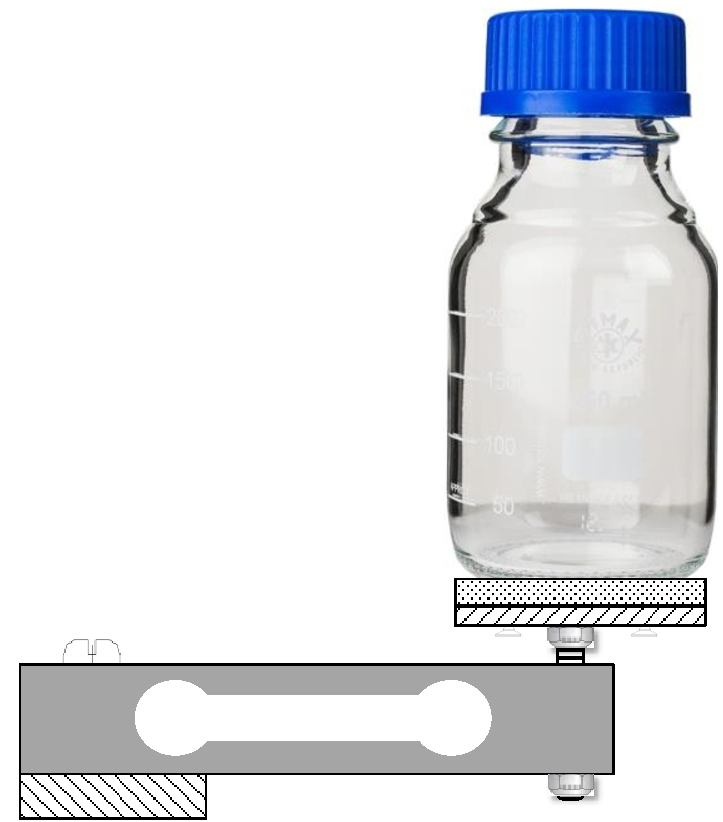
\includegraphics[width=0.5\textwidth]{billeder/Hardware/diagrammer/loadcell_montering.pdf}
	\caption{Illustration af opstilling med vægtcelle og celleopløsningsbeholder}
	\label{fig:loadcell_mont}
\end{figure}

\subsection{Kalibrering af vægtcellen}
Funktionen til vægtcellen er implementeret efter beskrivelsen i designdokumentet i projektdokumentation afsnit 4.3.5.3 \fxnote{Tjek ref}. Dens funktion er at konvertere det analoge input (V) til indholdet (ml) i celleopløsningsbeholderen. Dette er implementeret ved en lineær model:
\begin{align}
mL = a*input+b \text{, hvor a er hældningen og b er skæringen med y aksen}
\end{align}
Det analoge input ganges med en faktor \textit{a} plus et offset \textit{b} for at konvertere spænding til antal ml. Nedenstående tabel viser indgangsspændingen for forskellige mængder i beholderen. Udfra disse data er der lavet en lineær regression for at finde hældningen \textit{a} og skæringen \textit{b}.
\begin{center}
		\begin{longtable}{ | m{3cm} | m{3cm}| } 
			\hline
			\textbf{ml i beholder} &\textbf{Analog input} \\ 
			\hline
			 \SI{0}{\milli\litre} & \SI{1.9487}{\volt} \\ 
			\hline
			 \SI{25}{\milli\litre} & \SI{2.0440}{\volt} \\ 
			\hline
			\SI{50}{\milli\litre} & \SI{2.1320}{\volt} \\ 
			\hline
			\SI{75}{\milli\litre} & \SI{2.2297}{\volt} \\ 
			\hline
			\SI{100}{\milli\litre} & \SI{2.3109}{\volt} \\ 
			\hline
			\SI{125}{\milli\litre} & \SI{2.4071}{\volt} \\ 
			\hline
			\SI{150}{\milli\litre} & \SI{2.4961}{\volt} \\ 
			\hline
			\SI{175}{\milli\litre} & \SI{2.5821}{\volt} \\ 
			\hline
			\SI{200}{\milli\litre} & \SI{2.6760}{\volt} \\ 
			\hline
			\SI{225}{\milli\litre} & \SI{2.7654}{\volt} \\ 
			\hline
			\SI{250}{\milli\litre} & \SI{2.8587}{\volt} \\ 
			\hline
			\caption{Kalibreringsdata for vægtcellen}
			 		\end{longtable}
\end{center}

I Matlab er funktionen \textit{fitlm} anvendt til at finde det bedste lineære fit. Regressionen er baseret på Least Square metoden \citep{least}.
Udfra beregningerne i Matlab er hældningen a og skæringen b fundet til hhv:
\begin{align}
a = 276.14
\end{align}
\begin{align}
b = -539.02
\end{align}
Den endelige funktion er givet ved:
\begin{align}
ml = 276.140*input-539.02
\end{align}

Figur \ref{fig:loadcellcalib} viser den lineære funktion, samt de enkelte data punkter fra tabellen. 
\begin{figure}[H]
	\centering
	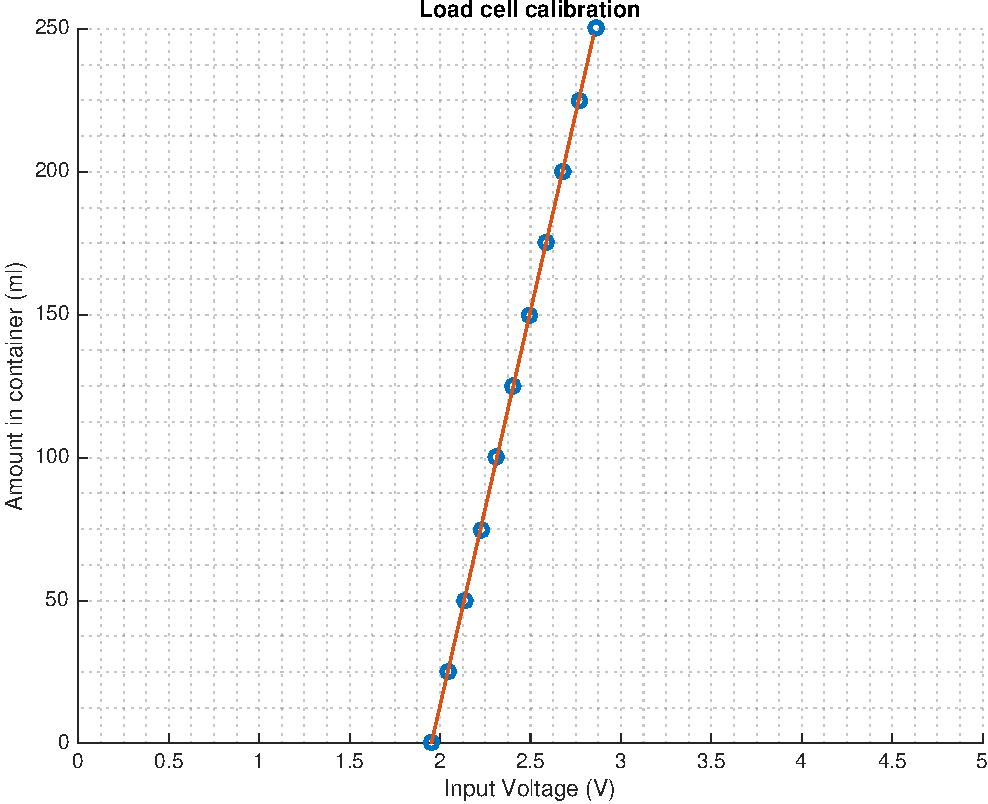
\includegraphics[width=0.6\textwidth]{billeder/software/calibration-crop.pdf}
	\caption{Kalibrering af load cell}
	\label{fig:loadcellcalib}
\end{figure}

For at reducere støj og mindske følsomheden overfor hurtigere ændringer i indgangsspændingen er der implementeret en midling af de seneste 10 målinger. Dette er med til, at gøre konverteringen mere robust overfor støj. 


\subsection{Integrationstest}
Til sidst i denne fase er der udført en integrationstest, hvor hardwaren er samlet, efter alle enkle enhedstest er udført. Efter samlingen af hardwaren er det verificeret at kredsløbet virker, hvorefter der er designet et PCB til samlingen af hardwaren. Derefter er integrationen med softwaren sket og igen er det verificeret, at det fungerer til en færdig prototype. 

